\chapter{Introduction}
\label{cha:intro}

This chapter describes a high level view of the SpiNNaker reasearch and its main uses. It highlights also the motivation and aims of my project and how it may impact on the improvement of a large scale international research.

\section{Overview}
\label{sec:overview}

"SpiNNaker is a biologically inspired, massively parallel computing engine designed to facilitate the modelling and simulation of large-scale spiking neural networks of up to a billion neurons and trillion synapses (inter-neuron connections) in biological real time." \cite{painkras} The SpiNNaker project, inspired by the fundamental structure and function of the human brain, began in 2005 and it is a collaboration between several universities and industrial partners: University of Manchester, University of Southampton, University of Cambridge, University of Sheffield, ARM Ltd, Silistix Ltd, Thales. \cite{spinnproject} A single SpiNNaker board is composed of hundreds of processing cores, allowing it to efficiently compute the interaction between populations of neurons, partially simulating a human brain.

\section{Project Aim}
\label{sec:aim}

This research project involves making use of the SpiNNaker software stack and hardware infrastructure, both optimised for neural network simulations, in order to explore and evaluate its usability and performance as a general purpose platform. This has been achieved through the development of a distributed Key-Value store and a Relational Database Management System with limited scope. 
This project has grown to be the largest non-neuromorphic application now available as part of the SpiNNaker API.

SpiNNaker is particularly strong at parallel execution at low power consumption, which appealed as an extraordinary opportunity to store and retrieve data in a fast, distributed way, under a database management system. This allows exploration of a broad range of ideas outside of the initial scope of SpiNNaker, testing some of its capabilities and limitations against a non-neuromorphic environment.

In addition to usability testing, an important objective is to gather performance benchmarks for this application, allowing analysis which can provide insights for improvements to the current architecture, possibly influencing on changes to reflect on the next generation of the chip: SpiNNaker 2. This data can also be used to further enhance my application in the future, as it is owned by the SpiNNaker team itself.

\section{SpiNNaker Architecture}

The basic building block of the SpiNNaker machine is the SpiNNaker Chip Multiprocessor (CMP), a custom designed globally asynchronous locally synchronous (GALS) system with 18 ARM968E-S processor nodes (figure \ref{fig:chip_layout}). \cite{painkras}
The SpiNNaker chip contains two silicon dies: the SpiNNaker die itself and a 128-MByte SDRAM (Synchronous Dynamic Random Access Memory) die, which is physically mounted on top of the SpiNNaker die and stitch-bonded to it (figure \ref{fig:spinn_dies}). \cite{spinnchip} The SDRAM serves as local shared memory for the 18 cores within the chip, also utilized for memory based communication. \cite{datasheet}

\begin{figure}
\centering
\begin{minipage}{.6\textwidth}
  \centering
  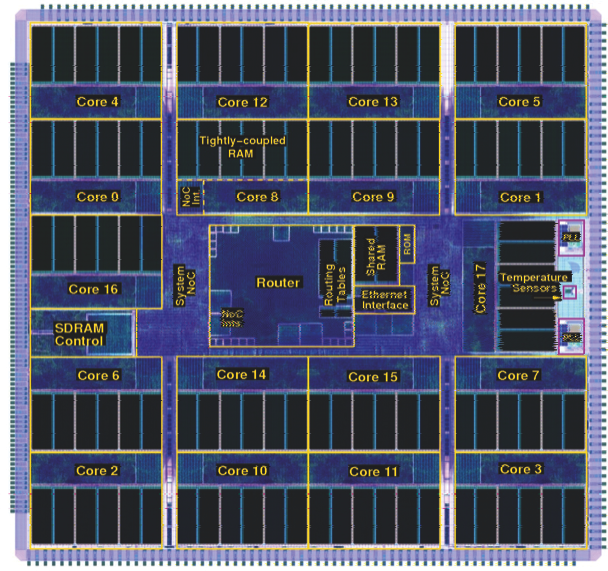
\includegraphics[width=1\linewidth, natwidth=608, natheight=571]{images/chip.png}
  \captionof{figure}{SpiNNaker chip layout}
  \label{fig:chip_layout}
\end{minipage}
\begin{minipage}{.3\textwidth}
  \centering
  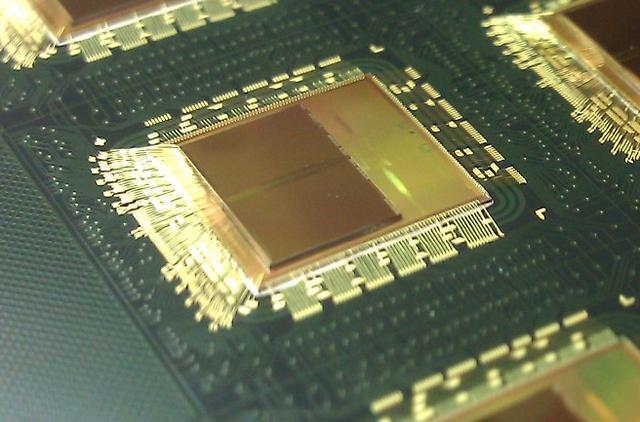
\includegraphics[width=1\linewidth, natwidth=640, natheight=422]{images/spinn_dies.jpg}
  \captionof{figure}{SpiNNaker CMP and SDRAM}
  \label{fig:spinn_dies}
\end{minipage}
\end{figure}

Each ARM core within the chip follows a 32-bit Harvard Architecture, holding a private 32-KB instruction tightly coupled memory (ITCM) and 64-KB data tightly coupled memory (DTCM).\cite{painkras} It has a small peak power consumption of 1-W at the nominal clock frequency of 180-MHz.\cite{arm968}

There are currently two types of SpiNNaker boards: \textbf{SpiNN-3} (figure \ref{fig:4node}), composed of 4 chips, thus a total of 72 processing cores, and \textbf{SpiNN-4} (figure \ref{fig:48node}), composed of 48 chips, this a total of 864 processing cores.

\begin{figure}
\centering
\begin{minipage}{.5\textwidth}
  \centering
  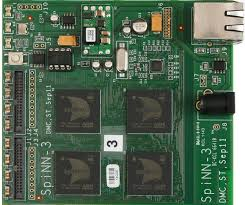
\includegraphics[width=0.4\linewidth, natwidth=245, natheight=205]{images/4node.jpg}
  \captionof{figure}{SpiNN-3}
  \label{fig:4node}
\end{minipage}%
\begin{minipage}{.5\textwidth}
  \centering
  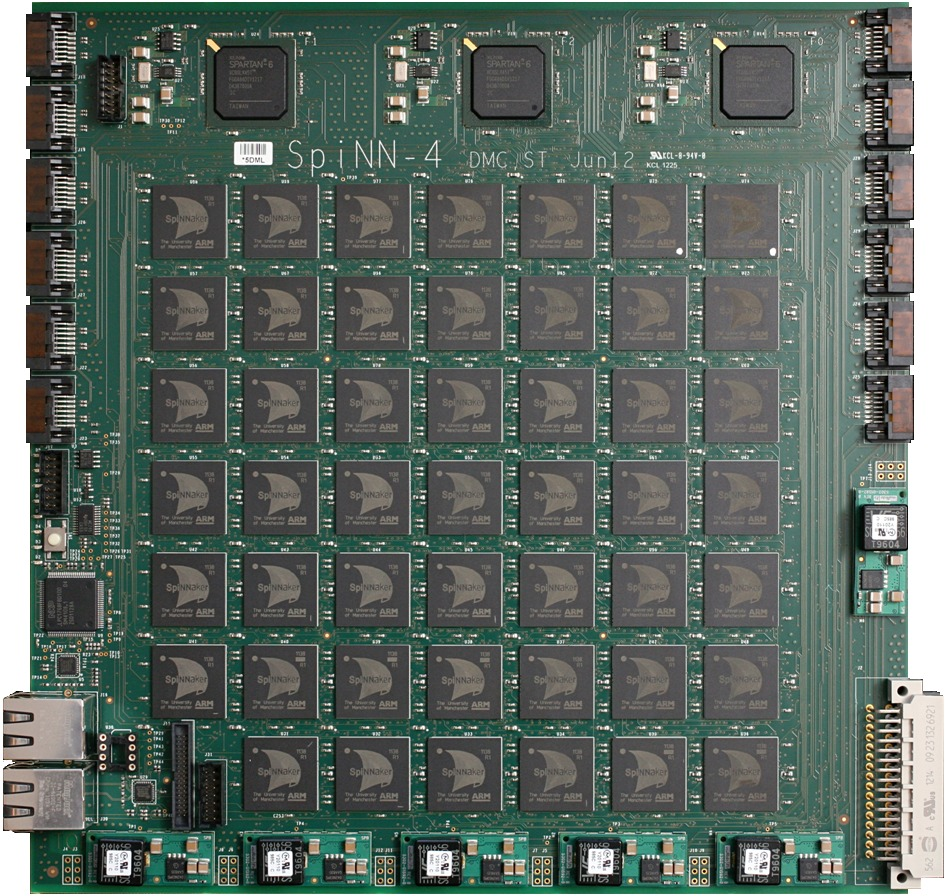
\includegraphics[width=0.9\linewidth, natwidth=945, natheight=896]{images/48node.jpg}
  \captionof{figure}{SpiNN-4}
  \label{fig:48node}
\end{minipage}
\end{figure}

\subsection{SpiNNaker Communication fabric}

The boards contain also a router, which manages inter-chip communication 


surrounded by a lightweight, packet-switched asynchronous communication infrastructure.

explain host computer, etc..


event driven architecture
donught shaped


XXXX should this be on the introduction???
event driven

The SpiNNaker API allows the utilisation of 4 different communication protocols between cores in the system. These packets trigger prioratised interrupts on the receiver, as it is an event driven architecture. These can be used to spread work load and transmit information initially private to a core.
It is worth noting that \textbf{none of these protocols guarantee successful delivery of data} and this effect is worsen if there is large traffic in the communication fabric. This means sending a large amount of packets symultaneously will result on packet drops.

\begin{itemize}
\item \textbf{Multicast (MC)}
The MC protocol, originally designed to simulate neural spikes, predicts a sigle source core casting a packet to multiple destinations. The packet contains only a 32 bit routing key, used by an external process to carry out the delivery, and an optional 32 bit payload, both provided at the source.

router.. routing table
\item \textbf{Point to Point (P2P)}
XXX
On top of the P2P layer, the SpiNNaker Datagram Protocol (SDP) was developed (build/written?) to allow larger transfers of data, of up to 280 (?) bytes, to reduce queueing on receival... (find the paper...)
%https://spinnaker.cs.man.ac.uk/tiki-download_wiki_attachment.php?attId=16

Using SDP, the SpiNNaker API XXX a User Datagram Protocol (UDP), allowing a two-way communication over IP addresses with the host machine. This allows uploading binaries and communicating back and forth with the hardware.

unreliability....
unreliable spikes (see that guy's paper...)

\item \textbf{Nearest-neighbour (NN)}
\item \textbf{Fixed-route (FR)}
\end{itemize}

[spinnaker datasheet page 30]

-mention DTCM only 64kb (so preferred to use SDRAM)
-look at your logbook for query plan stuff (at the start)
-debugging with ybug. testing with unit tests
-supported operations
-host is stateless
-tested on real data?

Each processor node on SpiNNaker includes a communication controller which is responsible for generating and receiving packets to and from the communication network.
The SpiNNaker architecture offers a range of...
all of which are unreliable!!

packet formats:


